
\section{Long-Ladder and Charge Division Tracking R\&D}

\subsection{Introduction}

The SiD collaboration has done microstrip R\&D in two directions that might provide attractive
alternatives to the SiD baseline: the exploration of the long-ladder limit for precision
microstrip tracking, and the exploration of the use of `charge division' -- reading out
resistive electrodes from both ends --
to glean information about the longitudinal position of the track
along the length of the sensor.

Two activities have been undertaken for the exploration of the long-ladder limit:
the development of an optimized, time-over-threshold readout ASIC (the LSTFE chip)
and a lab-bench study of the noise limitations associated with reading out long,
thin electrodes.
The possibility of using charge division to determine the longitudinal
coordinate of deposited charge with sub-centimeter precision was explored
using a mock electrode network read out with an optimized amplification and
shaping chain. Milestones have been achieved in all three areas.

\subsection{Recent Milestones}

The properties of this Long Shaping-Time Front End (LSTFE) microstrip readout ASIC have
been optimized for the readout of long ladders of silicon strip sensors that are motivated
by the need for precise low-mass central tracking for a Linear Collider Detector. With a
small and straightforward change to the shaping properties of the ASIC, it could be re-optimized
for use for the short strips and high occupancy that would be expected for ILC forward-tracking applications.
The LSTFE features optimized initial-amplification characteristics
and shaping time to reduce voltage-referenced readout noise, as appropriate for narrow-strip, long-ladder
applications. Unique to the LSTFE design, however, is the use of time-over-threshold readout to estimate the
analog pulse-height generated by subatomic particles passing through. A pulse-development and readout simulation developed
for the purpose of the designing the LSTFE suggests that the intrinsic statistical fluctuations of the
charge-deposition process in \unit[300]{\micron} of silicon obviate the need for a precise measurement
of deposited charge. A simulation of the centroid-finding (position-resolution) uncertainty provided by
time-over-threshold readout showed little degradation relative to that provided by an exact measurement of
deposited charge.

On the other hand, there are several advantages offered by the use of time-over-threshold readout. It is very simple
to implement within a digital back-end to the LSTFE's analog front end (the implementation would be on the same chip
as the front-end readout), requiring only a measurement of the number of clock counts that the given channel is over
threshold, and then the assembly and transmission of a
single data word containing the time of the upward transition, the time over threshold after the transition, and the
channel number. This happens in real time and is driven immediately off the chip into the DAQ, eliminating the need
for buffering and ADC conversion. In particular, there is no limit to the rate at which particles can be detected
other than the return-to-baseline of the analog signal, and so the data-accumulation rate capability of the device
is very high. In addition, for forward tracking, for which short strips are envisioned, the shaping time can be
shortened significantly. This will further improve the rate capability of the LSTFE readout, making it an excellent
choice for the high-occupancy forward region.
Figure~\ref{fig:Tracker:SCIPP:LSTFE} shows the fractional pulse-height uncertainty versus
injected charge achieved with the LSTFE front-end ASIC.

\begin{figure}
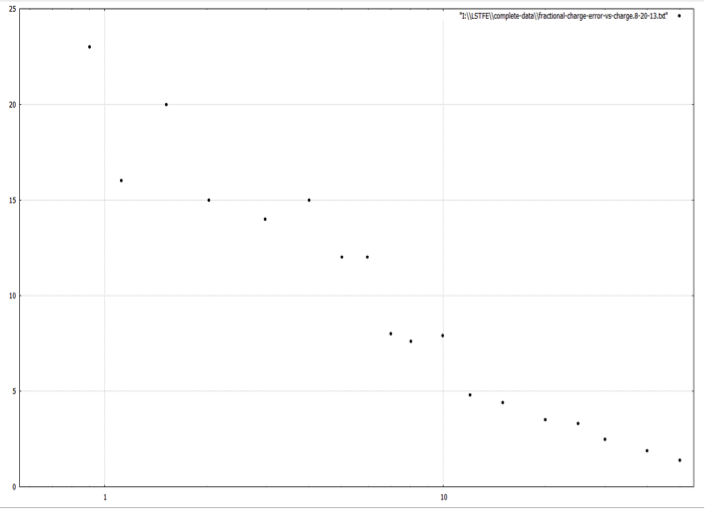
\includegraphics{Tracker/SCIPPTracking/SCIPPTracking}
\caption{Fractional pulse-height uncertainty (percent) versus injected charge (fC) for the LSTFE front-end ASIC.}
\label{fig:Tracker:SCIPP:LSTFE}
\end{figure}

The possibility of obtaining a longitudinal coordinate from silicon
microstrip sensors has been explored~\cite{Carman2011118}, making use of the
implant as a resistive electrode, with no overlain metallic electrode. An mock resistive
microstrip-implant electrode network was constructed on a PC board out of discrete resistors and capacitors
which was read out on both ends by an amplifying and shaping chain that was optimized to give the greatest
precision in the longitudinal position of the charge deposition on the implant. For a \unit[10]{cm}-long sensor,
a longitudinal resolution of \unit[6]{mm} was observed, achieving the resolution needed to aid in tracking
reconstruction in dense jet environments. Finally, sources of readout noise were measured and modeled
for sensors in the long, thin strip electrode limit~\cite{Collier2013127}. The readout noise observed
with the LSTFE ASIC was measured as a function of the length of a daisy-chained ladder of sensors,
and the results modeled with a SPICE simulation. It was found that network effects due to the
distributed resistance and capacitance of the electrode provide significant
mitigation of the readout noise relative to the assumption of single, lumped elements. It
was also found that reading out the ladder at its center rather than from one end provided
further noise suppression. Attaching this noise model to the pulse-development simulation
developed for the LSTFE design suggested that ladders of as much as \unit[75]{cm} long could be
made operation with end readout. Ladders approaching \unit[1]{m} in length could be operated with center readout.

\subsection{Engineering Challenges}

The primary remaining engineering challenges are the implementation of LSTFE power-cycling with a $\approx 1\%$
duty cycle, and the transfer of the digital back-end processing of the LSTFE information from
an off-chip FPGA directly onto the ASIC.

\subsection{Future Plans}

Because of this work, the possibility of a tracker making use of long ladders of silicon
microstrip sensors, or shorter strips with time-over-threshold readout in the forward
region, remains an option for the SiD detector. However, at this time resources are
being directed towards the modular KPiX design.

\subsection{Applications outside Linear Colliders}

It should be noted that the exploration of noise limitations for long, thin electrodes apply independently
of the sensor technology that generates the signals. Thus, this work may have
relevance to detection issues across a wide array of fields.


References
\begin{itemize}
\item \fullcite{Carman2011118}
\item \fullcite{Collier2013127}
\end{itemize}
